\documentclass[10pt,twocolumn]{article}

\usepackage{algorithm}
%\usepackage{moreverb}   
%\usepackage{longtable}
\usepackage{fancyhdr}
\usepackage{algorithmic}             
%\usepackage{algorithm}
%\usepackage{array}     
\usepackage{hyperref}
\usepackage{graphicx}
\usepackage{subfigure}
\usepackage{fullpage}
\usepackage{amsmath, amssymb, amsthm}
%\usepackage[framed,numbered,autolinebreaks,useliterate]{mcode}
%\usepackage{mathabx}

\usepackage{float}

\usepackage[margin=1in]{geometry}

\title{{\bf Intrusion Detection through Provenance-Based Histograms}}
\author{
    Kenny Yu\\
    Harvard University\\
    \href{mailto:kennyyu@college.harvard.edu}{\texttt{kennyyu@college.harvard.edu}}
  \and
    R. J. Aquino\\
    Harvard University\\
    \href{mailto:rjaquino@college.harvard.edu}{\texttt{rjaquino@college.harvard.edu}}
}
\date{CS261, Fall 2013}

\begin{document}

\maketitle

%%%%%%%%%%%%%%%%%%%%%%%%%%%%%%%%%%%%%%%%%%%%%%%%%%%%
% ABSTRACT
%

\begin{abstract}
Data-driven intrusion detection is a common system security technique. We present a histogram-based approach to intrusion detection, using provenance data generated by a provenance-aware storage system. By looking at simple provenance statistics and centrality metrics on provenance graphs, our approach identifies suspicious behavior based on deviations from prior normal system behavior. Our histogram-based approach requires no prior intuition about the types of exploits potentially being run on a system, and our analysis of two buffer overflow attacks and a modified version of \texttt{gcc} to log actions reveal which data is most useful in distinguishing between safe and malicious programs and program executions.
\end{abstract}

%%%%%%%%%%%%%%%%%%%%%%%%%%%%%%%%%%%%%%%%%%%%%%%%%%%%
% INTRODUCTION
%

\section{Introduction and Related Work}

\subsection{Provenance and PASS}

Provenance is metadata that tracks the history of all changes to files. In provenance-aware storage systems like PASS \cite{pass} and PASSv2 \cite{passv2}, the file system automatically tracks all dependencies whenever a file is created, modified, or deleted. These dependencies include the command that was executed to modify the file, the environment of the command, and all input files. The generated provenance forms a directed acyclic graph of typed nodes (e.g. files, processes, pipes) with properties (e.g. name, execution time, pid) and typed edges (e.g. forked, input, versioning). The edges show dependency, not data flow, and as a result, edges are directed from outputs to inputs. Table \ref{passobjects} indicates the types of objects the PASS tracks and attributes with those objects. PASS allocates pnode (``PASS" node) number and version numbers whenever PASS encounters a new object or a modification to an existing object. The combination of (pnode number, version number) uniquely identifies a node in our provenance graph. There are two versions of PASS. We conducted our experiments only with PASSv2; thus in this paper ``PASS" to refer to PASSv2.

\begin{table}[H]
\begin{center}
\begin{tabular}{|c|c|}
\hline
{\bf Node Types} & {\bf Description} \\
\hline
PROC & process \\
FILE & file \\
PIPE & pipe \\
NPFILE & non-PASS file \\
OTHER & other types of objects \\
\hline
{\bf Node Attributes} & {\bf Description} \\
\hline
INODE & inode of file \\
PATH & path of file \\
FREEZETIME & timestamp of record \\
CREAT & creation of file \\
UNLINK & unlinking file \\
EXECTIME & exec time of process\\
NAME & name of process \\
PID & pid of of process \\
ARGV & argument vector to process \\
ENV & environment of a process \\
\hline
{\bf Edge Types} & {\bf Description} \\
\hline
FORKPARENT & indicates parent PROC\\
&  of existing PROC node \\
INPUT & indicates input files\\
& or processes \\
VERSION & indicates a modification  \\
& to an existing node (e.g. \\
& modifying a file) \\
\hline
\end{tabular}
\end{center}
\label{passobjects}
\caption{Types of data collected by PASS}
\end{table}%

The PASS system automatically creates and updates provenance data for every file that was created or modified the volume. For example, the provenance for a data file that sent in a zip file would reveal both the name of the program that unzipped the file, as well as the web browser through which the zip file was downloaded! It is our belief that this level of specificity will lend itself to detecting patterns in program usage.

% TODO: The PASS system runs with minimal time overhead, and a reasonable space overhead (XXX cite real numbers).

To make sense of the large amounts of data, Macko et. al. have developed Orbiter, a tool to visualize provenance graphs with semantic zoom \cite{orbiter}. Margo et. al. have developed techniques to analyze large provenance graphs and to extract useful information from these graphs, including semantic file attributes \cite{fileattributes}. Using simple provenance statistics on nodes (e.g. neighbors, file count, process count, edge count) and features from \texttt{stat}, they determine with high accuracy the type of files (e.g. source files, configuration files). Furthermore, they have identified key properties of provenance graphs and developed new centrality metrics to perform local clustering of graphs, separating the huge provenance graphs into smaller semantic tasks or workloads \cite{clustering}.

\subsection{Intrusion Detection}

Applications that require provenance collection typically place great emphasis on data integrity. Given this priority, a natural goal of provenance systems is to detect intrusions on the system. Intrusion detection in live systems is a common problem in the systems community. There are two primary components to an intrusion detection system (IDS): (1) the data used to fuel the system's analysis, and (2) how the data is used.

Somayaji et. al. have developed techniques for detecting intrusions based on system call sequences, and their system counteracts these intrusions by exponentially delaying or aborting system calls, rendering the system useless for a malicious attacker \cite{somayaji}\cite{somayaji-recent}. Their system collects this data over a long period of "normal" time. If a process exhibits system call patterns that deviate from the ``normal" patterns for the process, their system flags it as potentially dangerous, and slows its execution. In this way, a program that continually deviates from normal behavior will be descheduled entirely. These intrusions include exploiting vulnerabilities in the SSH daemon and sendmail to obtain a shell with root privileges. Somayaji's work relies on building a {\em normal} profile of a process, and then detecting when the process deviates from normal.

Tariq et. al. generalize Somayaji's sequences of system calls to sequences of system events \cite{correlated-anomalies} to develop an IDS in a distributed system. Their system uses bloom filters to store hashes of $k$-tuples--representing a sequence of systemevents--and then use these bit vectors to correlate anomalies across multiple hosts back to the associated provenance. King et. al. have developed Backtracker \cite{backtracker}, a modified Linux kernel that tracks dependencies between operating system objects (files, processes, file names) in a similar fashion to PASS. Given an intrusion, Backtracker builds a backwards casual graph to determine the entry point of an intrusion, and they have extended Backtracker with forward causal graphs to determine possibly tainted files, processes, and hosts from an intrusion in a distributed system \cite{multihost}. However, their system does not have a way of detecting an intrusion. Lei et. al. build similar process-file dependency trees, which they call access trees, and define a compatibility function to compare access trees with the goal of predicting future file accesses based on the current access tree pattern \cite{fileprefetch}.

Despite the existing work to detect intrusions and anomalies, Cao et. al. argue that any intrusion detection system cannot always distinguish good behaviors from bad behaviors because users behave too randomly to have an accurate model of the user's behavior \cite{fuzzy}. They propose their fuzzy anomaly detection approach to extend the training models in existing intrusion detection systems to account for the inherent fuzzy nature of intrusion detection. When training an IDS, instead of assigning hard 0s or 1s for features, their approach provides a way to reliably map these features to weights in the interval $[0,1]$. 

\subsection{Our Goals and Contributions}

Given the extensive amount of data PASS collects on file-file, file-process, and process-process dependencies and existing work in intrusion detection that uses these kinds of directed graphs of files and process data, it seems plausible to detect intrusions based on provenance data collected by PASS. In particular, we hope to answer the questions:
\begin{itemize}
\item Given PASS provenance data, what kinds of intrusions can be detected?
\item What provenance data is most useful for detecting these kinds of intrusions.
\end{itemize}

Our system is designed to run offline, so we run our algorithms on the full set of provenance data. While this approach is slower than running an online system like Somayaji and Tariq, it allows us to take in the full picture of the events during a process's execution, without having to preselect the information we think will be useful. This approach is especially helpful because different information leads to the detection of different types of intrusions. The data collected by Backtracker's dependency graph of process and files is very similar to the data PASS generates, and their exploits and analysis techniques directly inspired our work. 

In this paper, we present a histogram-based technique for analyzing existing PASS provenance data to detect if an intrusion occurred. To detect intrusions, we generate statistical models of normal behavior, against which we can test a node of interest. These statistical models are histograms of different graph statistics, and we use these histograms to generate kernel density estimations to evaluate a test node. The lower the kernel density estimate, the less ``normal" the node. 

We hypothesize that intrusions are deviations from normal behavior, and these deviations are likely to manifest themselves in different number of inputs,  outputs, and centrality counts. We chose to use histograms because histograms are easy and fast to make, and if this approach works well, can be turned into an online method for detecting intrusions as the system is running.

The contributions of this paper are:
\begin{enumerate}
\item A histogram-based technique for using provenance data to detect intrusions
\item An analysis of the different intrusions that can be identified, and the types of provenance which best contribute to these detections
\item Future extensions to our work to create better intrusion detection models and make more use of provenance data
\end{enumerate}


%%%%%%%%%%%%%%%%%%%%%%%%%%%%%%%%%%%%%%%%%%%%%%%%%%%%
% DESIGN
%

\section{Design and Implementation}
Here we present our intrusion detection technique: a general and extendable statistical method for analyzing and comparing provenance data. At a high level, we create a provenance data graph and generate a model of ``normal" behavior for each process/file in the graph. Using this model, we can determine the likelihood that a given ``test" deviates from normal behavior and is thus potentially an exploited or malicious program.
\subsection{Models}
Our approach requires statistical models to evaluate the normalcy of a test node. The statistical model we chose to use was a kernel density estimation (KDE), which estimates the probability density function of a value with unknown distribution. To create the KDE, we needed to provide counts of a particular statistic. For each statistic:
\begin{enumerate}
\item We computed the counts for that statistic over all the nodes in the provenance graph.
\item We aggregated the counts by the NAME field of the node (e.g. the path to a file for a FILE node, or path to an executable for PROC node). For objects with no NAME field (e.g. PIPE objects), we used the tuple of (pnode number, VERSION number) as the node's name.
\item For each unique name in the graph, we use the counts on that name to generate a histogram of ``normal" behavior. We convert these histograms into kernel density objects to smoothen our histogram and generalize to all continuous values for the statistic.
\end{enumerate}

This model allows us to evaluate a test node's normalcy according to that statistic. For example, we could then ask ``Does node $X'$ have a statistically believable number of output processes compared to the other $X$ nodes?"

\subsection{Provenance Statistics}
We expected intrusions to differ in terms of the statistics that would stand out, and as a result, we needed to generate a diverse suite of statistics and a model for each. For our simple provenance graph statistics, we compiled the following statistics:
\begin{enumerate}
\item The number of input files to the node.
\item The number of input processes to the node.
\item The number of input pipes to the node.
\item The number of output files to the node.
\item The number of output processes to the node.
\item The number of output pipes to the node.
\item The number of VERSION edges into this node.
\item The number of VERSION edges out of this node.
\end{enumerate}
For ease of computation and comparison, we treated the different node types (e.g. file, process, pipe) separately so that we can treat, for instance, "input files to a file node" and "input files to a process node" as separate counts.

\subsection{Centrality Metrics}
In addition to the data that can be collected on the nodes directly, we computed centrality metrics on the nodes using the centrality metrics proposed by Macko et. al. \cite{clustering}. In their work, they noted 3 properties of provenance graphs:
\begin{enumerate}
\item The ubiquity (importance) of a node is a function of a node's descendants, not its ancestors. (Note: Because edges in provenance graphs are in the direction of data dependence instead of data flow, ``descendants" in this case means data flow descendants and NOT descendants by traversing provenance graph edges).
\item There is no agreed-upon granularity in which provenance should be captured.
\item Provenance has a temporal component.
\end{enumerate}

Using these observations, they propose several centrality metrics on provenance graphs:
\begin{itemize}
\item \textbf{In-degree Centrality}. Because a node's importance is based on its output descendants, then the number of times a node was used as input to another node indicates a simple measure of importance.
\item \textbf{Age}. They note that large "jumps" in timestamps or age might indicate breaks between tasks, but this interpretation is complicated when scripts execute tasks in short succession.
\item \textbf{Ancestor Centrality}. This measures the total number of descendants of a node, normalized by the total number of nodes in a graph.
\item \textbf{Opsahl's Closeness Centrality}. This accounts for the number of edges between a node and its descendants. To compute this, we calculate
$$CC'(v) = \sum_{x \in V -  \{v\}} (d'_{xv})^{-1}$$
where $d'_{xv}$ is the distance from node $x$ to $v$ by only following outgoing edges from $x$. Unreachable nodes from $x$ will have $d'_{xv} = \infty$, and so $(d'_{xv})^{-1} = 0$.
\item \textbf{Provenance Eigenvector Centrality}. The centrality of the nodes is given by the left dominant eigenvector of the matrix:
$$M_{ij} =
\begin{cases}
1 & \text{if there is an edge } i \to j \\
1/|V| & \text{if there is no out edge from } i \\
0 & \text{otherwise}
\end{cases}
$$
\end{itemize}

We each metric, we computed the centrality of all the nodes and aggregated the counts by name to generate our histogram and kernel density estimations like the simple statistics we used above.

\subsection{Implementation}
We used Orbiter \cite{orbiter} to visualize and examine the provenance graphs. We wrote Python scripts to (1) parse the raw BerkeleyDB database files storing the PASS data (2) build the provenance graphs (3) collect the counts for each statistic (which include running the centrality calculations), and (4) optionally outputting the histograms and kernel density estimations for a node of interest in a second provenance graph. We should note here that some centrality calculations proved difficult to run efficiently on large provenance graphs, particularly the Eigenvector Centrality mentioned above. As such, it is not included in our below analyses. 

\subsection{Examples}
In Figure 1, we see a few examples of a generated histogram and KDE model. The green bars represent the histogram for the particular statistic, and the blue curve is the KDE. Finally, the red line is the value for a ``test" node. In this case, the test node appears to be a possible exploit, because it intersects the KDE at low values. 
\begin{figure*}
  \label{kde-example}
  \caption{Example histograms of a centrality measure and process statistic for the \texttt{gcc} exploit, with the associated KDE. The green bars represent the raw histogram counts, the blue curve represents the kernel density function, and the red vertical line represents the estimation of a node of interest.}
  \centering
    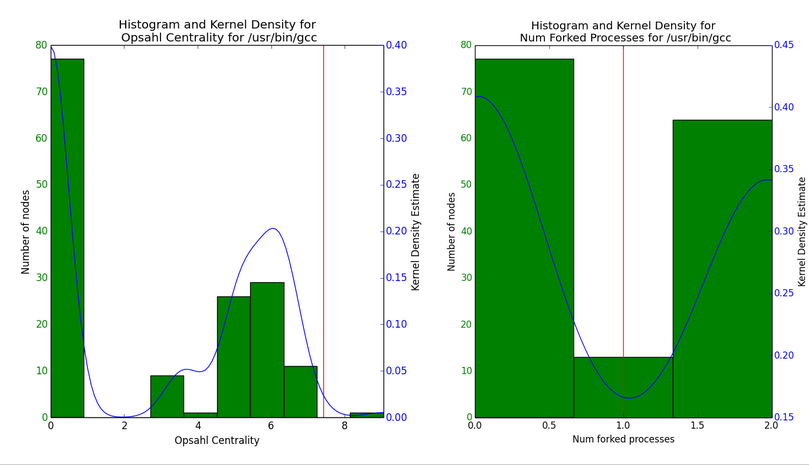
\includegraphics[width=\textwidth]{img/hist.png}
\end{figure*}


%%%%%%%%%%%%%%%%%%%%%%%%%%%%%%%%%%%%%%%%%%%%%%%%%%%%
% EVALUATION
%

\section{Evaluation}

\subsection{Evaluation Methodology}
In order to test our techniques, we needed to run exploits on our PASS-enabled machine. We looked to prior work to get a sense of the different types of techniques commonly used to exploit security vulnerabilities. Commonly, remote network techniques (as seen in Backtracker \cite{backtracker}) are used to breach insecure systems. Metasploit \cite{metasploit} is a software package designed to facilitate running exploits on insecure system. Searching the Metasploit database, as well as the online Exploit Database \cite{exploitdb}, we found that most successful techniques involve exploiting vulnerabilities in software that a target system is running, as opposed to vulnerabilities in the target system itself. Put another way, we sought to exploit software packages, like mcrypt and gcc, not the Linux kernel itself. 

To generate the provenance data necessary to run the analyses, we needed to run both good and exploited versions of our programs.

\subsubsection{hello}
We found that many of the popular exploits involved buffer overflows and arbitrary code execution. Programming bugs in a piece of software allowed a malicious user, sending well-crafted data, to run arbitrary code on the target system. We created a simple \texttt{hello} program that echos standard in to standard out, and we gave it a buffer overflow vulnerability that allows a malicious user to fork a process. 

We ran \texttt{hello} normally 40 times on various inputs and collected the provenance times. We then exploited the buffer overflow vulnerability in \texttt{hello} to spawn an \texttt{ls} process, and saved the standard out of that process to a file. See Figure 2 for provenance graphs displaying normal and exploited behavior of \texttt{hello}.

\subsubsection{mcrypt}
The mcrypt encryption package had a long standing buffer overflow, which would allow a malicious user to run their own code when mcrypt tried to decrypt the crafted exploit file. Due to limitations in our Virtual Machine set up, we were unable to exploit the vulnerable version of mcrypt, much like the authors of Backtracker \cite{backtracker} found. To emulate this exploit, we designed a Python program, which would decrypt (via ROT13) an input file. When sent a particular exploit file� which contained malicious lines, our program would stop decrypting and start running the code specified in the file.

We ran our program on over 200 good inputs, and stored the provenance data. We then ran our program on two bad inputs, first to call \texttt{ls} as a Proof of Concept, and again to call \texttt{/bin/sh} to demonstrate that more severe attacks can be performed. We again exported the provenance generated by these steps, for comparison with our good usage. This is similar to recording all uses of a program during a server's lifetime. See Figure 3 displaying normal and exploited behavior for our version of mcrypt.

\subsubsection{gcc}
Another type of exploit is more reminiscent of a system administration failure. If a malicious user replaces a program in \texttt{/usr/bin}, it could be used to log user actions. To emulate this sort of attack, we replaced \texttt{/usr/bin/gcc} with our own version of gcc, which, in addition to compiling the user's code (via a call to gcc), logs that the user has made a request and copies the files the user had tried to compile. 

For our system administration attack, we compiled the PASS toolset using GCC, and exported the provenance from these runs. We then replaced GCC with our exploited version, compiled the toolset several times with different configurations, and exported the provenance again. In this way, we collected provenance for normal usage and from our exploited usage.
\begin{figure*}
  \label{hello-orbiter}
  \caption{Descendants of a \texttt{hello} program. The top image shows multiple invocations of a \texttt{hello} behaving normally when invoked with \texttt{cat foo.txt | ./hello > c.txt}. The bottom image shows \texttt{hello} being exploited to fork an \texttt{ls} process.} 
  \centering
    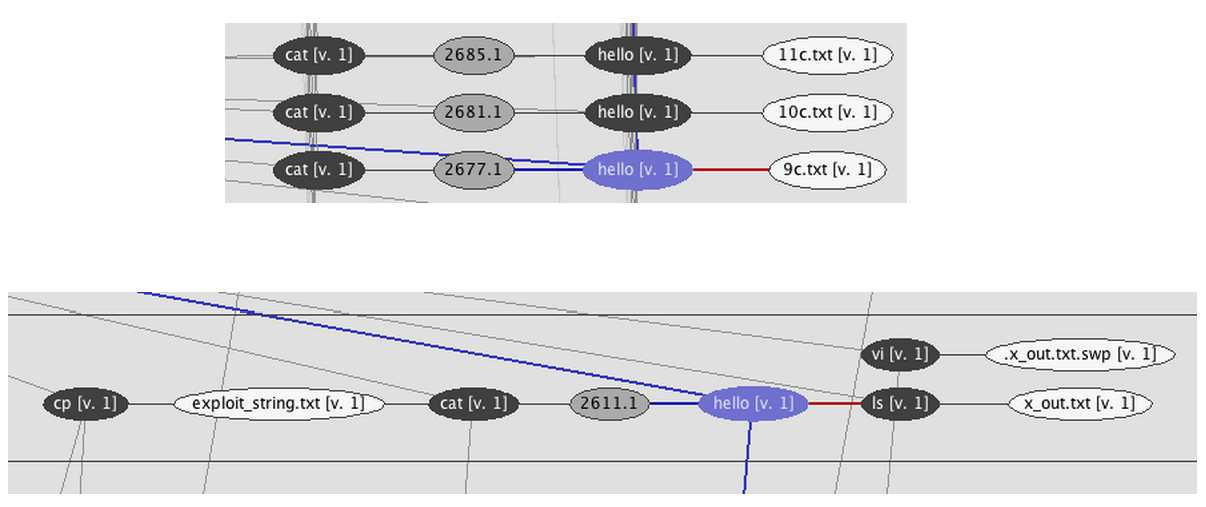
\includegraphics[width=\textwidth]{img/hello.png}
\end{figure*}
\begin{figure*}
  \label{mcrypt-orbiter}
  \caption{Descendants of an unexploited mcrypt-style program. Simply an output file. Below, descendants of an exploited mcrypt-style program. In addition to an (offscreen) output file, there is also an outgoing \texttt{/bin/sh} process, with its own children.}
  \centering
    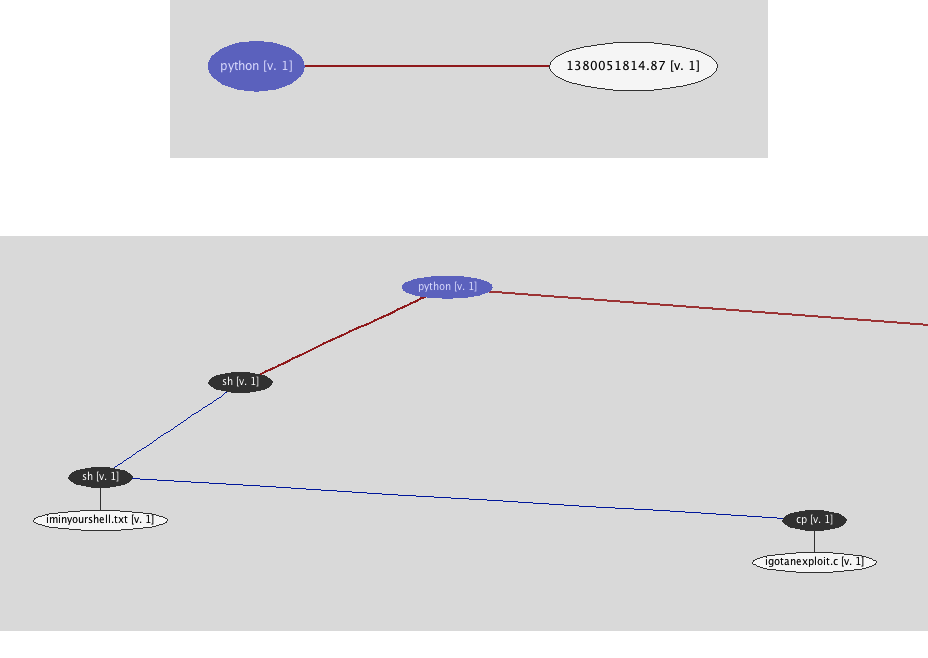
\includegraphics[width=\textwidth]{img/mcrypt.png}
\end{figure*}

\subsection{Selecting Metrics}
Because we had no prior intuition into what the histograms on provenance data would actually look like, we approached selecting statistics from an objective, data-based standpoint. We wanted to use statistics that had variation over our workload to minimize the dependency of our statistics on the workload data. Towards this end, we graphed all of the statistics over the ``normal" provenance data, to see where there were trends and variation. Our results for GCC are in Figures 4 and 5. We can see that proc\_out\_proc (outgoing processes), the ancestor centrality, and Opsahl Closeness Centrality statistics have more variation, whereas the other statistics were unimodal or bimodal (0 or 1). 

The unimodal and bimodal statistics would not generate useful kernel density estimates, as they would predict roughly 0.5 for either a 0 or 1 count, giving us no information about whether the node in question is behaving normally.  On the other hand, the statistics with more variation in data would actually provide more useful information when determining normalcy in new test nodes. As we include more data (as discussed in Future Work), these sorts of graphs will become increasingly important in selecting good statistics for evaluation.
\begin{figure*}
  \label{simple-gcc}
  \caption{Histograms over all "simple" provenance statistics for GCC}
  \centering
    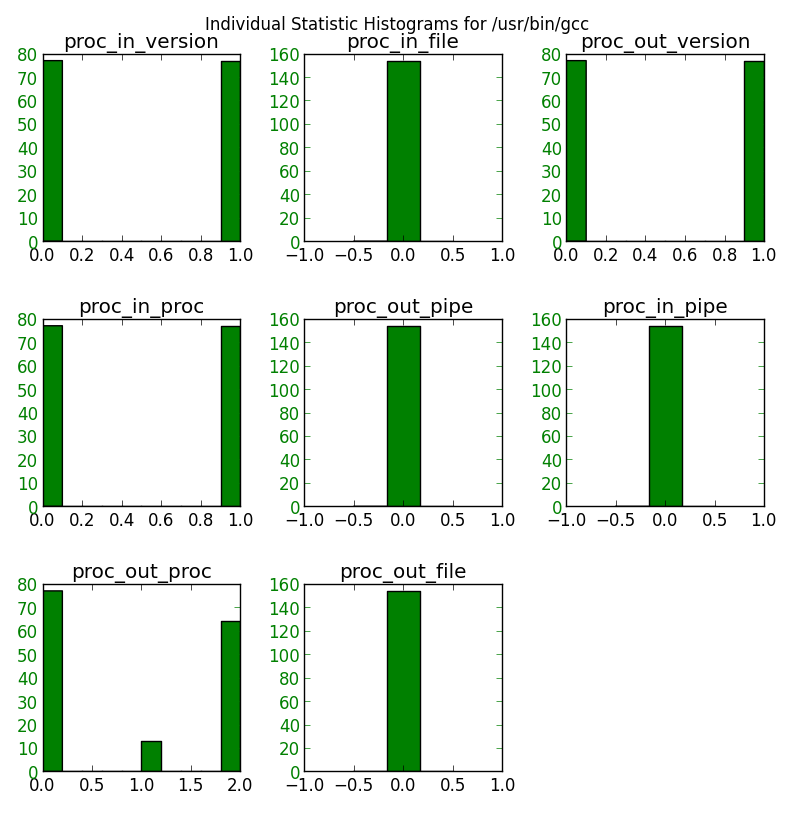
\includegraphics[width=0.7\textwidth]{img/gcc_stats.png}
\end{figure*}
\begin{figure*}
  \label{centrality-gcc}
  \caption{Histograms over all centrality metrics for GCC}
  \centering
    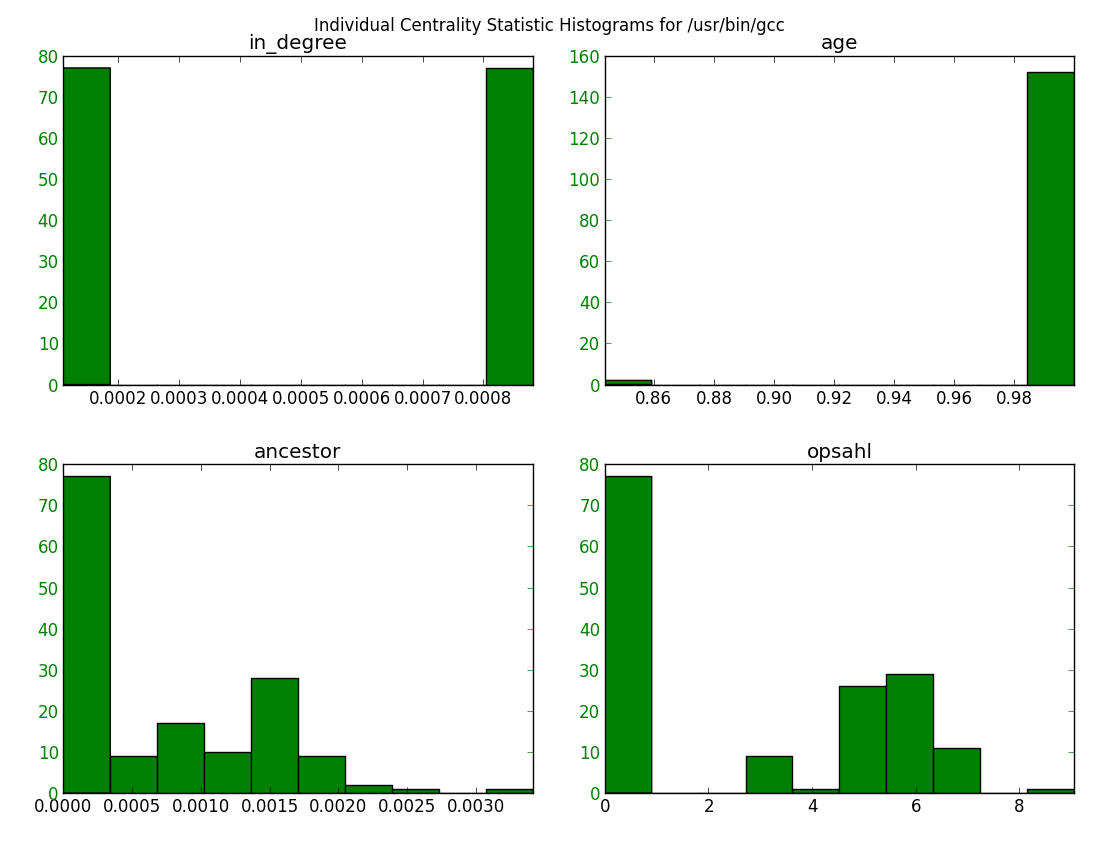
\includegraphics[width=0.7\textwidth]{img/gcc_cent_stats.png}
\end{figure*}


\section{Results}
\subsection{Provenance Data}
After running the normal and exploited programs described above, we visualized the provenance graphs using Orbiter \cite{orbiter}. After searching for the nodes named after our programs, we were able to find both the clean and exploited nodes. The clean nodes for ``hello" simply read in one file through a pipe and outputted one file, whereas the exploited version clearly has a forked \texttt{/usr/bin/ls} process. Similarly, the mcrypt simulation (implemented in Python) has only an output file as a descendent normally, but when exploited has multiple extra processes/files as descendants (see Figure 2 and Figure 3). Similarly, the normal GCC and exploited GCC displayed very different provenance graphs, but they were too big to fit legibly on a page.


\subsection{Statistical Data and KDE Predictions}
Table 2 summarizes some of the preliminary results we have generated. Here we have included, for each statistic and test, the average over the "normal" nodes, the observed value for the "test" node, and the KDE probability output for that value. We have chosen four metrics that provided a statistically significant result. 
% The other statistics failed to be as powerful (see Table 2 XXX).
% from http://hhh123.wordpress.com/2008/08/13/latex-table-across-two-columns/
% TODO: include difference/ratio from normal?
\begin{table*}[ht]
\label{results}
{\small
  \begin{center}
  \begin{tabular}{| l | l | l | l |}
    \hline
    metric & hello & mcrypt & gcc \\ \hline
     \# forked processes & 0.0 | 1 | 0.108 & 0.0 | 1 | 0.107 & 0.9 | 0 | 0.408 \\ \hline
     \# input files & 0.5 | 0 | 0.453 & 0.5 | 0 | 0.453 & 0.5 | 1 | 0.107 \\ \hline
     \# output files & 0.5 | 1 | 0.453 & 0.5 | 1 | 0.453 & 0.0 | 3 | 0.000 \\ \hline
    Opsahl centrality & 1.791 | 2.83 | 0.252 & 1.250 | 4.867 | 0.000 & 2.793 | 7.415 | 0.024 \\ \hline
    %Ancestor centrality & 0.0009 | 0.0011 | 0.799 & 0.0002 | 0.0014 | 0.798 & 0.0007 | 0.0002 | 0.798 \\

    \hline
  \end{tabular}
  \end{center}
}
\hfill{}
\caption{average over good | test node value | kernel density estimate of test node being ``normal"
}
\label{tb:tablename}
\end{table*}
\subsection{Discrimination/False Positives}
We were initially concerned that while our methods would reveal exploited nodes, they would also flag ``normal'' nodes as potential exploits. To determine whether this was the case, we ran our analyses on the ``normal'' nodes. To determine the worst possible outcome, here we report the minimum KDE value that a ``good'' node produced for a given test. If this value is significantly lower than the value we saw for a ``bad'' node, we can be reasonably confident in the power of that test. This method should also be investigated as a means for automatically determining thresholds for ``bad'' nodes. 

In Table 3, we report, for each exploit, the minimum KDE value we saw for a ``normal'' node, along with the number of nodes examined. Comparing these values to the values shown in Table 2 confirms our belief that these metrics can distinguish between ``normal'' and abnormal nodes. One exception is that of outgoing processes for gcc, where the minimum node was far below even the exploit node. The node in question only had one outgoing process, where most nodes (as shown in Figure 1) had 0 or 2. As shown in the histogram, there were nodes with this odd value. The node in question had normal values for the other metrics, however, so a combined view would not have necessarily flagged the node as abnormal. These combined metrics must be developed so as to minimize false positives and maximize true positives.
\begin{table*}[ht]
\label{results}
{\small
  \begin{center}
  \begin{tabular}{| l | l | l | l |}
    \hline
    metric & hello (80 nodes) & mcrypt (424) & gcc (154) \\ \hline
     \# forked processes & 0.453 & 0.798 & 0.166\\ \hline
     \# input processes &  0.617 & 0.453 & 0.453\\ \hline

     \# input files & 0.453 & 0.453 & 0.798\\ \hline
     \# output files &  0.453 & 0.798 & 0.798\\ \hline

     \# input pipes & 0.798 & 0.798 & 0.798\\ \hline
     \# output pipes &  0.798 & 0.798 & 0.798\\ \hline

    \hline
  \end{tabular}
  \end{center}
}
\hfill{}
\caption{minimum kernel density estimate of test node being ``normal" seen on a ``normal'' node. With few exceptions, these values are high.
}
\label{tb:tablename}
\end{table*}

\section{Discussion}
\subsection{Successes}
We were able to accurately identify our three exploited programs. Each was a slightly different exploit, but each exploit deviated enough on some metrics which flagged them as non-normal. 

\subsection{Useful Data for Intrusion Detection}
We set out to identify both buffer overflows (i.e. arbitrary code execution) and modified binaries. The buffer overflows were best detected by the number of outgoing processes and the centrality measures. This makes sense, as arbitrary code execution will generate additional processes. Of the centrality metrics we implemented, the Opsahl Centrality metric did the best in distinguishing an exploited node from normally behaving nodes. Because the Opsahl Centrality metric accounts for the number of edges between a node and all of its descendants, this centrality metric is very sensitive to the addition of nodes. Exploits that have additional outputs (e.g. new processes and output files through a remote shell), thus generate a higher Opsahl centrality metric for the offending node. The more active the exploit is (say, if it forks a user shell), the more the centrality measure will be impacted, and the more likely it is that the exploit will be caught by our model.

If the exploit does directly not generate additional files, however, statistics like "number of output files" will fail to be statistically significant. Indeed, the two programs (hello and mcrypt) that did not generate additional files were not flagged by that measure. On the other hand, the GCC that was modified to generate log files was caught by this measure, as it generated many more files than a normal GCC process. 

\subsection{Confusing Data Patterns}
At first, some of the data we collected seemed wrong. Why, for instance, does GCC seem to normally output zero files? Upon further inspection, we found that GCC forks processes for the linker/assembler that handles generating output, so GCC does not directly have output files. Similarly, when running a python script, the code file itself is not directly executed, it is read in by a python process, which then goes off and collects input, generates output, and forks additional processes. Thus, when running a python file, the file itself only has one node in the provenance graph, with many python process nodes accessing it. To run our analyses, we needed to manually identify this connection, and compute statistics for the python process, instead of the single code file node.

%%%%%%%%%%%%%%%%%%%%%%%%%%%%%%%%%%%%%%%%%%%%%%%%%%%%
% CONCLUSION
%

\section{Future Work}
\subsection{N-depth Statistics}
Currently, the statistics and counts we generate apply only to the test node itself. As mentioned above, some processes fork helper processes that take in input or generate output, which would be useful information to collect. In order to account for these sorts of actions, we could calculate the relevant statistics for the test node and all nodes at distance $N$ from the test node, and then aggregate them. We could experiment with aggregation techniques to determine how best to incorporate this information. Perhaps it is best to simply sum all neighbor statistics together, or perhaps this information calls for new histogram and model. By utilizing information about neighboring nodes, we hope to see an increase in accuracy and the ability to detect less blatant intrusions.

Additionally, by using this approach, we could avoid the manual process identification mentioned above. On python files, for instance, N-depth statistics would compute statistics for the python process, which is always a direct neighbor of the code file we initially cared about.

\subsection{Histograms by Name}
Currently, our system compute statistics based on node type, but not node name. For instance, When we compute the outgoing (i.e. "forked") processes, we simply count them. Thus, if a program normally forks something benign, like say \texttt{cp}, but an exploited version forks \texttt{rm}, the raw counts may not reveal this (a call to \texttt{/bin/sh}, however, should impact the centrality measures). One direction to attempt to rectify this problem lies in generating more specific histograms. Instead of having a model for "number of processes forked", we could generate one model per type of process forked, e.g. "number of \texttt{cp} processes forked". This more specific data might enable us to catch intrusions in larger programs that already modify a lot of files and fork a lot of processes.
\subsection{ENV and ARGV}
Currently we ignore the environment and argument information stored in the provenance graph. By generating histograms based on this information, we could catch subtler intrusions/exploits that rely on modified environment information. Additionally, if an exploit relies on a particular argument or argument patterns, this information might reflected in the ARGV information.
\subsection{Parameters}
Currently, constructing the kernel density estimates requires a few parameter decisions - namely the number/size of the bins for our histograms, as well as the bandwidth parameter for constructing the KDE. We, for the purposes of this experiment, modified these parameters manually until they described the data well, but we could computer optimal values programmatically, or test out multiple values. Additionally, we demonstrated that odd behavior has a ``low" KDE, but we did not define what ``low" means. For this system to be deployed more widely, we will need to define or compute what thresholds signify a potential intrusion or exploit.
\subsection{Online Intrusion Detection}
Currently, this system runs after-the-fact. We can identify intrusions that occurred on a machine by analyzing the data after it has been lifted from the target machine. Because PASS collect data in real time, however, our approach can be modified to implement online intrusion detection. To achieve this goal, we would need to only use metrics that can be updated without recomputing the entire statistic. In particular, some of the centrality measures do not meet this criterion. We would also need to add additional daemons (or modify the existing PASS daemons) to run the appropriate statistic gathering and model generating code. Another extension is to apply progressive versions of our centrality metrics, including a progressive form of PageRank which computes the importance of a node online.
\subsection{Local vs. Global}
In our experiments, we looked at provenance graphs in their entirety. However, provenance graphs are meant to be long-lived, and an intrusion that affected only a small portion of the graph will have negligible effects on the global structure of the graph. To resolve this issue, a possible future extension to our work is to cluster the nodes based on time \cite{clustering} and then only examine the most ``recent" nodes when applying our histogram technique.
\section{Conclusion}
We have demonstrated that provenance data (in this case, data generated by PASS) can be used to identify anomalies in program behavior, which often signal a security intrusion or exploit. Using provenance-based histograms, we can construct models of the regular usage patterns for a particular program. When the intrusion or exploit results in behavior deviating from these models, its provenance allows us to flag it as a potential intrusion. Replaced binaries that acted significantly differently were especially easy to detect. Histograms on simple provenance statistics are good for identifying simple anomalies, but more complex statistics (see future work) may enable us to detect subtler intrusions.

%%%%%%%%%%%%%%%%%%%%%%%%%%%%%%%%%%%%%%%%%%%%%%%%%%%%
% BIBLIOGRAPHY
%

\begin{thebibliography}{99}

\bibitem{fuzzy}
\textsc{Cao, D., Qiu, M., Chen, Z., Hu, F., Zhu, Y., and Wang, B.} Intelligent Fuzzy Anomaly Detection of Malicious Software. In {\em Internal Journal of Advanced Intelligence}, vol. 4, no. 1, pp 69-86 (December 2012).

\bibitem{somayaji-recent}
\textsc{Inoue, H. and Somayaji, A.} Lookahead Pairs and Full Sequences: A Tale of Two Anomaly Detection Methods. In {\em 2nd Annual Symposium on Information Assurance} (June 2007). 

\bibitem{backtracker}
\textsc{King, S. T. and Chen, P. M.} Backtracking Intrusions. In {\em SOSP'03 Proceedings of the nineteenth ACM symposium on Operating systems principles} (December 2003).

\bibitem{multihost}
\textsc{King, S. T., Mao Z. M., Lucchetti, D. G., and Chen, P. M.} Enriching intrusion alerts through multi-host causality. In {\em Proceedings of the 2005 Network and Distributed System Security Symposium} (February 2005).

\bibitem{fileprefetch}
\textsc{Lei, H. and Duchamp, D.} An Analytical Approach to File Prefetching. In {\em Proceedings of the USENIX 1997 Annual Technical Conference} (January 1997).

\bibitem{clustering}
\textsc{Macko, P., Margo, D., Seltzer, M.} Local Clustering in Provenance Graphs (Extended Version). In {\em Proceedings of the 22nd ACM international conference on Conference on information \& knowledge management} (August 2013).

\bibitem{orbiter}
\textsc{Macko, P. and Seltzer, M.} Provenance Map Orbiter: Interactive Exploration of Large Provenance Graphs. In {\em TaPP'11 Proceedings of the 2nd conference on Theory and practice of provenance} (June 2011).

\bibitem{fileattributes}
\textsc{Margo, D., and Smogor, R.} Using Provenance to Extract Semantic File Attributes. In {\em TaPP'10 Proceedings of the 2nd conference on Theory and practice of provenance} (February 2010).

\bibitem{passv2}
\textsc{Muniswamy-Reddy, K., Braun, U., Holland, D. A., Macko, P., Maclean, D., Margo, D., Seltzer, M., and Smogor, R.} Layering in Provenance Systems. In {\em Proceedings of the 2009 USENIX Annual Technical Conference} (June 2009).

\bibitem{pass}
\textsc{Muniswamy-Reddy, K., Holland, D. A., Braun, U., and Seltzer, M.} Provenance-Aware Storage Systems. In {\em Proceedings of the 2006 USENIX Annual Technical Conference} (June 2006).

\bibitem{exploitdb}
\textsc{Offensive Security, Inc.} The Exploit Database. {\tt http://www.exploit-db.com}.

\bibitem{metasploit}
\textsc{Rapid 7 Inc.} Metasploit Framework. {\tt http://www.metasploit.com}.

\bibitem{somayaji}
\textsc{Somayaji, A. and Forrest, S.} Automated Response Using System-Call Delays. In {\em Proceedings of the 2000 USENIX Annual Technical Conference} (August 2000).

\bibitem{correlated-anomalies}
\textsc{Tariq, D., Baig, B., Gehani, A., Mahmood, S., Tahir, R., Aqil, A., and Zaffar, F.} Identifying the provenance of correlated anomalies. In {\em SAC'11 Proceedings of the 2011 ACM Symposium on Applied Computing} (March 2011).

\end{thebibliography}

\end{document}
